\documentclass[aspectratio=169,10pt]{beamer}
\usepackage[utf8]{inputenc}
\usepackage{amsmath, amsfonts}
\usepackage{graphicx}
\usepackage{lmodern}
\usepackage{tikz}
\usepackage{pgfplots}
\usepackage{enumitem}
\setlist[itemize]{noitemsep,topsep=2pt,partopsep=0pt,parsep=0pt,leftmargin=*}
\renewcommand{\familydefault}{\sfdefault}
\pgfplotsset{compat=1.18}

\title{Model Calibration: Platt Scaling and Isotonic Regression}
\author{}
\date{}

\setbeamercolor{frametitle}{fg=blue!70!black}
\setbeamercolor{title}{fg=blue!70!black}
\setbeamerfont{frametitle}{series=\bfseries}
\setbeamertemplate{navigation symbols}{}
\setlength{\abovedisplayskip}{4pt}
\setlength{\belowdisplayskip}{4pt}
\begin{document}

\begin{frame}[t]
\titlepage
\end{frame}

% ------------------------------------------------------------
\begin{frame}[t]{Model Calibration: Definition, Workflow, and Curve}
\begin{columns}[T,onlytextwidth]

\column{0.52\textwidth}
\textbf{What is model calibration?}
\begin{itemize}
\item Calibration aligns predicted probabilities with empirical frequencies.
\item Customer example: 100 customers with predicted churn 0.7 should yield ~70 churns.
\item If 80 churn, the model is \textbf{underestimating} risk.
\item If 50 churn, the model is \textbf{overestimating} risk.
\end{itemize}

\textbf{Workflow (steps)}
\begin{itemize}
\item Train base model on training data.
\item Predict on validation (calibration) set.
\item Fit calibration map (Platt or Isotonic).
\item Apply map to test and future data.
\end{itemize}

\textbf{Goal}
\begin{itemize}
\item Improve probability quality without hurting ranking too much.
\end{itemize}

\column{0.48\textwidth}
\textbf{Calibration curve}
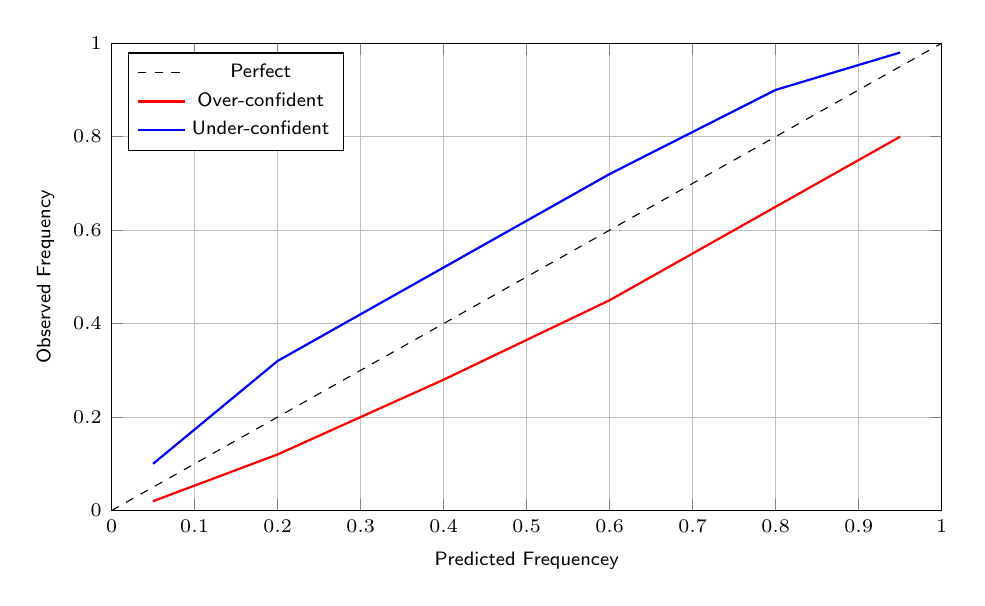
\begin{tikzpicture}
\begin{axis}[
    width=\linewidth,
    height=0.62\linewidth,
    xmin=0, xmax=1,
    ymin=0, ymax=1,
    xlabel={Predicted Frequencey},
    ylabel={Observed Frequency},
    grid=both,
    tick label style={font=\scriptsize},
    label style={font=\scriptsize},
    legend style={at={(0.02,0.98)},anchor=north west, font=\scriptsize},
]
\addplot[dashed, black] coordinates {(0,0) (1,1)};
\addlegendentry{Perfect}
\addplot[thick, red] coordinates {(0.05,0.02) (0.2,0.12) (0.4,0.28) (0.6,0.45) (0.8,0.65) (0.95,0.80)};
\addlegendentry{Over-confident}
\addplot[thick, blue] coordinates {(0.05,0.10) (0.2,0.32) (0.4,0.52) (0.6,0.72) (0.8,0.90) (0.95,0.98)};
\addlegendentry{Under-confident}
\end{axis}
\end{tikzpicture}

\textbf{Interpretation}
\begin{itemize}
\item On-diagonal: calibrated.
\item Below: over-confident.
\item Above: under-confident.
\end{itemize}

\end{columns}
\end{frame}

% ------------------------------------------------------------
\begin{frame}[t]{Brier Score,Reliability & Resolution}
\begin{columns}[T,onlytextwidth]

\column{0.55\textwidth}
\textbf{Brier score}
\[
\text{Brier} = \frac{1}{N} \sum_{i=1}^{N} (p_i - y_i)^2
\]
\small
Lower is better. Decomposes into reliability, resolution, and uncertainty.

\[
\text{Brier} = \text{Reliability} - (\text{Resolution} + \text{Uncertainty})
\]

\[
\text{Reliability} = \sum_{b=1}^{B} \frac{n_b}{N} (p_b - \hat{y}_b)^2
\]

\[
\text{Resolution} = \sum_{b=1}^{B} \frac{n_b}{N} (\hat{y}_b - \hat{y})^2
\]

\[
\text{Uncertainty} = \hat{y} (1 - \hat{y})
\]

\column{0.45\textwidth}
\textbf{Term definitions}
\begin{itemize}
\item $N$: number of samples.
\item $p_i$: predicted probability for sample $i$.
\item $y_i$: true label for sample $i$ (0/1).
\item $B$: number of probability bins.
\item $n_b$: number of samples in bin $b$.
\item $p_b$: mean predicted probability in bin $b$.
\item $\hat{y}_b$: empirical positive rate in bin $b$.
\item $\hat{y}$: overall positive rate.
\end{itemize}

\textbf{Intuition}
\begin{itemize}
\item Reliability: closeness of predicted probs to observed rates within bins.
\item Resolution: how far bin-wise observed rates deviate from the overall rate.
\item Uncertainty: irreducible variance from base rate $\hat{y}$.
\end{itemize}

\end{columns}
\end{frame}

% ------------------------------------------------------------


% ------------------------------------------------------------
\begin{frame}[t]{Platt Scaling: Process and Math}
\begin{columns}[T,onlytextwidth]

\column{0.55\textwidth}
\textbf{Idea}
\begin{itemize}
\item Fit a sigmoid to map uncalibrated scores to probabilities.
\item Works well when miscalibration is roughly sigmoidal.
\end{itemize}

\textbf{Math}
\[
P_{\text{cal}} = \frac{1}{1+\exp(Af + B)}
\]
\begin{itemize}
\item $f$: uncalibrated score or probability.
\item $A, B$: learned on validation set.
\end{itemize}

\column{0.45\textwidth}
\textbf{Process}
\begin{itemize}
\item Train base model on train set.
\item Get $f$ on validation set.
\item Fit logistic regression with $f$ as input.
\item Apply sigmoid to test and future data.
\end{itemize}

\textbf{Pros / Cons}
\begin{itemize}
\item Pros: stable on small datasets; low variance.
\item Cons: limited to sigmoid-shaped corrections.
\end{itemize}

\end{columns}
\end{frame}

% ------------------------------------------------------------
\begin{frame}[t,shrink=8]{Isotonic Regression: Idea and Algorithm}
\begin{columns}[T,onlytextwidth]

\column{0.6\textwidth}
\textbf{Idea}
\begin{itemize}
\item Learn a monotone, piecewise-constant mapping.
\item No parametric shape assumptions.
\end{itemize}

\textbf{Objective}
\[
\min_{\hat{y}} \sum_{i=1}^{n} (y_i - \hat{y}_i)^2
\quad \text{s.t. } \hat{y}_1 \le \hat{y}_2 \le \cdots \le \hat{y}_n
\]
\small
\textit{$\hat{y}_i$ are the \textbf{uncalibrated} predicted probabilities (scores) sorted by value.}

\textbf{Block averaging}
\[
\hat{y}_B = \frac{1}{|B|} \sum_{i \in B} y_i
\]

\textbf{Example (sorted by score)}
\scriptsize
\resizebox{0.60\linewidth}{!}{%
\begin{tabular}{c c c}
\hline
Score $\hat{y}$ & True $y$ & Calibrated Score \\
\hline
0.10 & 0 & 0.10 \\
0.20 & 1 & 0.20 \\
0.30 & 0 & 0.25 \\
0.40 & 1 & 0.25 \\
0.60 & 1 & 0.60 \\
\hline
\end{tabular}%
}
\normalsize


\column{0.4\textwidth}
\textbf{PAV algorithm (merge blocks)}
\begin{itemize}
\item Start with each point as its own block.
\item Scan left-to-right for violations ($v_i > v_{i+1}$).
\item Merge violating blocks and replace with weighted average.
\item Repeat until monotonic.
\end{itemize}

\textbf{Calibrated probabilities}
\begin{itemize}
\item Fit isotonic map on validation set.
\item Transform base model scores on test/future data.
\end{itemize}

\end{columns}
\end{frame}

% ------------------------------------------------------------


\end{document}
